% Drawing 150/01-3 -- folder 150, batch 01, archive page 9 (PDF page 10).
% Transcription: seul dessin de la page : en haut, « $X_2^{*}$ » ; un disque au centre duquel un point marqué « $\underline{X}_0 = X_0^{*}$ » ; un rayon du centre à un point épais du bord, marqué « $X_{01}$ », prolongé hors du disque par une demi-droite épaisse marquée « $\underline{X}_1$ » ; de part et d'autre, deux demi-droites parallèles issues du bord, marquées « $X_{12}$ ».
% Kind: disc with a centre, a radius and three parallel half-lines. Method 2 (schematic redraw from the facsimile). Status: ok.
% Notes: A closed curve (the disc) with a marked point at its centre, labelled X_0 = X_0^* (the first X underlined); a radius from the centre to a heavy point on the boundary, labelled X_{01} under it; from that point a heavy half-line going right, labelled X_1 (underlined; the index is written over a blot, and the transcription suggests X_1^* as a doubtful reading: X_1 is kept); above and below, two thinner half-lines starting on the boundary, each labelled X_{12}; X_2^* above the disc. The radius, the heavy point and the three half-lines start at points computed on the boundary curve. The same figure as the left drawing of p. 6 (01-2), in the notation of the X. The printed listing showing through from the back of the sheet is not drawn. Overlaid 2026-11-12 (Opus 5.5) on a 400 dpi colour render: disc, centre, half-lines and labels match the page within about a unit; nothing corrected. Redrawn 2026-11-12 (issue 128): to check again.
% Coordinates: 1 unit = 1 mm = 1/100 of the crop width (bbox in page fractions: [0.24, 0.075, 0.56, 0.22]).
% Redrawn by Claude (claude-fable-5-2), issue #128, 2026-11-12; not checked by a human; not compiled (no TeX in the session).
% Overlaid by Claude (claude-opus-5-5) 2026-11-12 (issue #128): rasterised from its own coordinates over the colour facsimile and checked or corrected. Not compiled. Status: ok.
% Rights: reproduces part of the work -- behind RENDER_TRANSCRIPTS, never published by itself.
\documentclass[tikz,border=3pt]{standalone}
\usepackage{amsmath,amssymb}
\usetikzlibrary{patterns,arrows.meta,calc}
\tikzset{pencil/.style={black!45}, struck/.style={black!35}, mpt/.style={circle,draw,inner sep=1.3pt}, pt/.style={circle,fill,inner sep=0.9pt}, opt/.style={circle,draw,fill=white,inner sep=1.1pt}}
\begin{document}
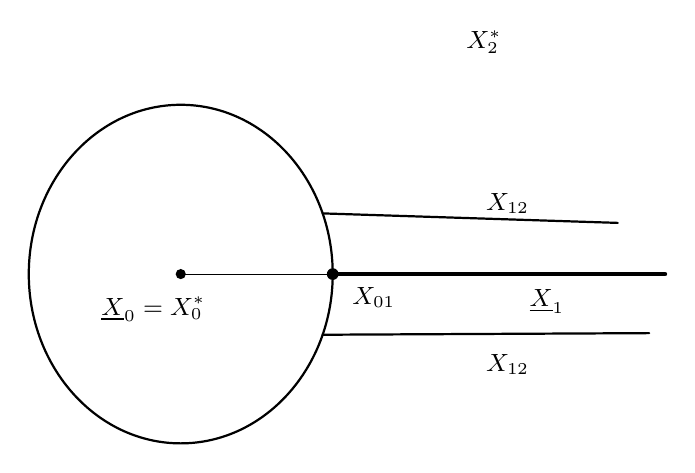
\begin{tikzpicture}[x=1mm,y=1mm,line cap=round,line join=round,font=\scriptsize]
\coordinate (O) at (25.5,-37.5);
\draw[thick] (O) ellipse [x radius=19.3, y radius=21.5];
\coordinate (P) at ($(O)+(0:19.3 and 21.5)$);
\coordinate (U) at ($(O)+(21:19.3 and 21.5)$);
\coordinate (L) at ($(O)+(-21:19.3 and 21.5)$);
\draw (O) -- (P);
\draw[ultra thick] (P) -- (87,-37.5);
\draw[thick] (U) -- (81,-31);
\draw[thick] (L) -- (85,-45);
\node[pt,inner sep=1.3pt] at (O) {};
\node[pt,inner sep=1.5pt] at (P) {};
\node[inner sep=1pt] at (64,-8) {\small $X_2^{*}$};
\node[inner sep=1pt] at (22,-42) {\small $\underline{X}_0 = X_0^{*}$};
\node[inner sep=1pt] at (50,-40.5) {\small $X_{01}$};
\node[inner sep=1pt] at (72,-41) {\small $\underline{X}_1$};
\node[inner sep=1pt] at (67,-28.5) {\small $X_{12}$};
\node[inner sep=1pt] at (67,-49) {\small $X_{12}$};
\end{tikzpicture}
\end{document}
